
	Avec les chapitres~\deux et~\trois nous avons appris à quantifier les transferts d’énergie, mais nous ne pouvons le faire que si l’on connaît les valeurs de $u$ ou de $h$, des propriétés qu’il est impossible de mesurer directement en pratique.
	
	Ce \coursquatre se propose de répondre à deux questions :
	\begin{itemize}
		\item Comment peut-on décrire le comportement de l’air losqu’on le chauffe ou le comprime ?
		\item Comment peut-on prévoir les valeurs de $u$ et de $h$ lorsqu’on utilise de l’air ?
	\end{itemize}
	Ce chapitre est incompatible avec le \courscinq, où nous devrons oublier tout ce qui est appris ici. \dontbreakpage \vspace{2em}


\section{Définition}

	\subsection{Le manomètre comme thermomètre}
	\label{ch_le_manomètre_comme_thermomètre}

		Nous retiendrons de prime abord la définition suivante :

		\begin{trucimportant}
			Le gaz parfait est un \textit{modèle mathématique},\linebreak
			permettant de prédire la température d’un gaz en fonction de sa pression.
		\end{trucimportant}

		Le gaz parfait est une proposition de définition de la température. On propose simplement de mesurer la température absolue $T$ avec un manomètre, en stipulant qu’elle est directement proportionnelle à la pression $p$ et inversement proportionnelle à la masse volumique $\rho$.

		On peut ainsi dire que le gaz parfait ne décrit pas la réalité des choses, que ce n’est pas un principe physique, mais bien simplement un modèle simplifié du comportement des gaz. Sa plage de validité est limitée et floue.



		\subsection{Définition : l’équation d’état}

		Nous appellerons \vocab{gaz parfait} un fluide à l’état gazeux dont le multiple de la pression et du volume, $p v$ , reste proportionnel à sa température. La constante de proportionnalité est nommée \vocab{constante du gaz}, et notée $R$ ; elle dépend de la nature du gaz.

		\begin{equation}
			p v = R T
			\label{eq_pv=RT}
		\end{equation}

		\begin{equationterms}
			\item par définition pour un gaz parfait,
			\item où \tab $p$ \tab est la pression (\si{\pascal}),
			\item \tab $v$ \tab le volume spécifique (\si{\metre\cubed\per\kilogram}),
			\item \tab $T$ \tab la température (\si{\kelvin}),
			\item et \tab $R$ \tab la constante du gaz considéré (\si{\joule\per\kelvin\per\kilogram}).
		\end{equationterms}

		L’\cref{eq_pv=RT} est nommée \vocab{équation d’état des gaz parfaits}. Elle peut également être exprimée en fonction de la masse :
		\begin{equation}
			p V = m R T
			\label{eq_pV=mRT}
		\end{equation}
		
		\begin{equationterms}
			\item où \tab $V$ \tab est le volume (\si{\metre\cubed}),
			\item et \tab $m$ \tab la masse de gaz considérée (\si{\kilogram}).
		\end{equationterms}

		Parce qu’elle est étroitement liée à la définition de la température (pour laquelle elle définit un degré zéro), il a fallu 150 ans pour que cette équation prenne sa forme définitive, telle qu’énoncée par \wf{Émile Clapeyron} en 1834.


	\subsection{Que représente un gaz parfait ?}
	\label{ch_gaz_parfait_kezako}

		Le gaz parfait est le modèle le plus simple que l’on puisse imaginer pour représenter le comportement d’un gaz.
		
		Selon ce modèle, les molécules se comportent comme des sphères rebondissant les unes contre les autres (\cref{fig_gaz_boules}). On peut imaginer un grand nombre de très petites boules de billard en mouvement chaotique, qui se percutent et rebondissent les unes contre les autres sans jamais s’attirer ni dissiper leur énergie par frottement.
		
		\begin{figure}
			\begin{center}
				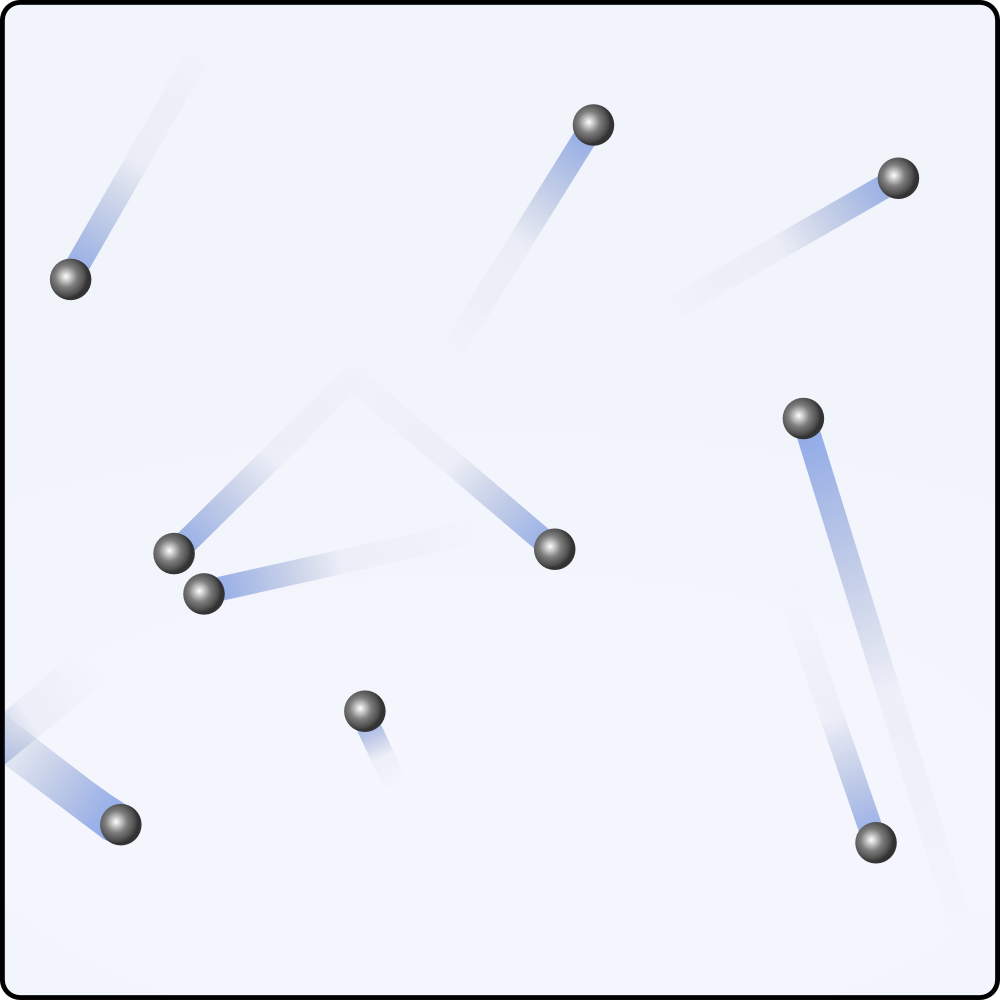
\includegraphics[width=8cm]{images/gaz_boules.png}
			\end{center}
			\supercaption{Un gaz parfait peut être visualisé comme un ensemble de boules en mouvement désordonné. Elles se percutent sans frottement et sans attraction mutuelle. La vitesse de chaque boule change à chaque heurt.}%
			{Dérivé d’\wcfile{Kinetic_theory_of_gases.svg}{un schéma} \ccbysa par \wcu{Sharayanan}}
			\label{fig_gaz_boules}
		\end{figure}
		
		Dans ce chaos, la température est une mesure de l’énergie cinétique des molécules. On la quantifie en mesurant la force résultant de l’impact des molécules sur une paroi du récipient --\ c’est-à-dire avec la pression. Avec ce modèle, nous pouvons proposer une échelle de température telle que $T \propto p$.
		
		Maintenant, pour générer une pression donnée, plus le nombre de molécules impactant la surface est faible, et plus il faut qu’elles l’impactent fortement. Ainsi, lorsque la masse volumique $\rho$ diminue à une pression donnée, c’est que la température augmente. On peut donc également proposer $T \propto \frac{1}{\rho}$.
		
		Traduisons ces deux propositions en une équation, et nous obtenons un modèle simple pour quantifier la température : $T \propto p v$.
		
		
	\subsection{Que ne représente pas un gaz parfait ?}
	\label{ch_pas_gaz_parfait}		
		
		Le comportement réel des molécules lorsqu’elles sont proches les unes des autres est en réalité très complexe, car les forces d’attraction y jouent un rôle déterminant. L’influence de ces forces d’attraction augmente aussi lorsque les molécules sont structurellement complexes\footnote{Ainsi par exemple, l’interaction entre deux molécules d’hydrocarbone est plus difficile à modéliser que l’interaction entre deux molécules d’hélium.} et lentes.

		Les conséquences à l’échelle macroscopique de ces interactions, et les conditions dans lesquelles elles ne sont plus négligeables, font l’objet du \courscinq.

		Nous retiendrons pour l’instant que le modèle du gaz parfait fonctionne mieux :

		\begin{itemize}
			\item Lorsque les molécules se percutent à grande vitesse, c’est-à-dire que la température du gaz est haute ;
			\item Lorsque l’espace moyen entre les molécules est grand, c’est-à-dire lorsque le volume spécifique du gaz est grand.
		\end{itemize}
		
		Ces conditions permettent de s’assurer que les forces d’attraction entre molécules gardent un rôle mineur dans le comportement global du gaz. Elles sont respectées pour l’air dans la grande majorité des applications en ingénierie. Nous utiliserons la valeur $R_\text{air} = \SI{287}{\joule\per\kilogram\per\kelvin}$ pour l’air pur dans nos machines.


	\subsection{Limites du modèle}

		Il ne faudra pas longtemps à l’étudiant/e pour trouver les limites de l’\cref{eq_pV=mRT}, qui indique qu’une masse non-nulle de gaz parfait occupe \textit{un volume nul} à température nulle. Strictement parlant, le gaz parfait ne peut exister --\ le modèle mathématique ci-haut perd son sens à très basse température puisqu’il ne tient pas compte du volume des molécules lui-même.

		Plusieurs autres équations d’état peuvent être utilisées pour correspondre aux gaz réels sur une plus grande plage de propriétés.

		Ainsi, l’équation de \textit{Van der Waals}, proposée dès la fin du \textsc{xviii}\ieme siècle, est formulée selon :
		\begin{equation}
			\left(p + \frac{a}{v ^2}\right) (v - b) = R T
		\end{equation}
		
		\begin{equationterms}
			\item où $a$ et $b$ sont deux constantes.
		\end{equationterms}

		Cette équation a l’intérêt de tenir compte de deux facteurs ignorés dans l’équation d’état~\ref{eq_pV=mRT} : la force d’attraction entre les molécules (le terme $a/v^2$, qui devient partie de l’expression de la pression) et le volume occupé par les molécules elles-mêmes (le terme $b$ qui se retranche au volume disponible).

		Malgré les difficultés inhérentes à la quantification des termes $a$ et  $b$, ces modifications ont considérablement étendu la plage d’application des équations d’état. Elles ont valu à leur auteur, \wf{Johannes Diderik van der Waals}, le prix Nobel de physique en 1910.

		La recherche de modèles mathématiques pour décrire l’état des gaz réels est un thème important de recherche en mécanique des fluides. L’étudiant/e curieux/se pourra consulter les équations d’état \wed{Real_gas\#Beattie.E2.80.93Bridgman_model}{de Beattie-Bridgeman}, \wed{Benedict\%E2\%80\%93Webb\%E2\%80\%93Rubin_equation}{de Benedict-Webb-Rubin} ou encore de Strobridge pour se faire un aperçu de la complexité croissante de cette branche. Nous resterons quant à nous à l’\cref{eq_pv=RT}.



\section{Propriétés des gaz parfaits}

	\subsection{Deux capacités calorifiques importantes}

		Nous avons déjà abordé la notion de capacité calorifique (ou «~chaleur massique~»), au premier chapitre (\ref{eq_def_capacité_calorifique_massique}). Elle se définit comme la quantité de chaleur nécessaire pour augmenter d’un Kelvin\footnote{Ou d’un degré Celsius, ces différences de température étant égales.}
		la température d’un kilo du corps. On a ainsi :
		\begin{equation}
			c = \frac{\diff q}{\diff T}
		\end{equation}
		
		\begin{equationterms}
			\item où \tab $c$ \tab est la capacité calorifique spécifique (\si{\joule\per\kelvin\per\kilogram}),
			\item \tab $\diff q$ \tab la quantité infinitésimale de chaleur spécifique fournie (\si{\joule\per\kilogram}),
			\item et \tab $\diff T$ \tab la variation infinitésimale de température provoquée (\si{\kelvin}).
		\end{equationterms}

		Comme la température d’un gaz varie aussi lorsqu’il reçoit ou fournit du travail, il existe une infinité de façons de faire varier sa température d’un degré, en combinant chaleur et travail (\cref{fig_expérience_diff_chaleurs_massiques}). Chacune nécessite une quantité de chaleur unique ; il y a donc \textit{une infinité de chaleurs massiques} correspondantes. 

		\begin{figure}
			\begin{center}
				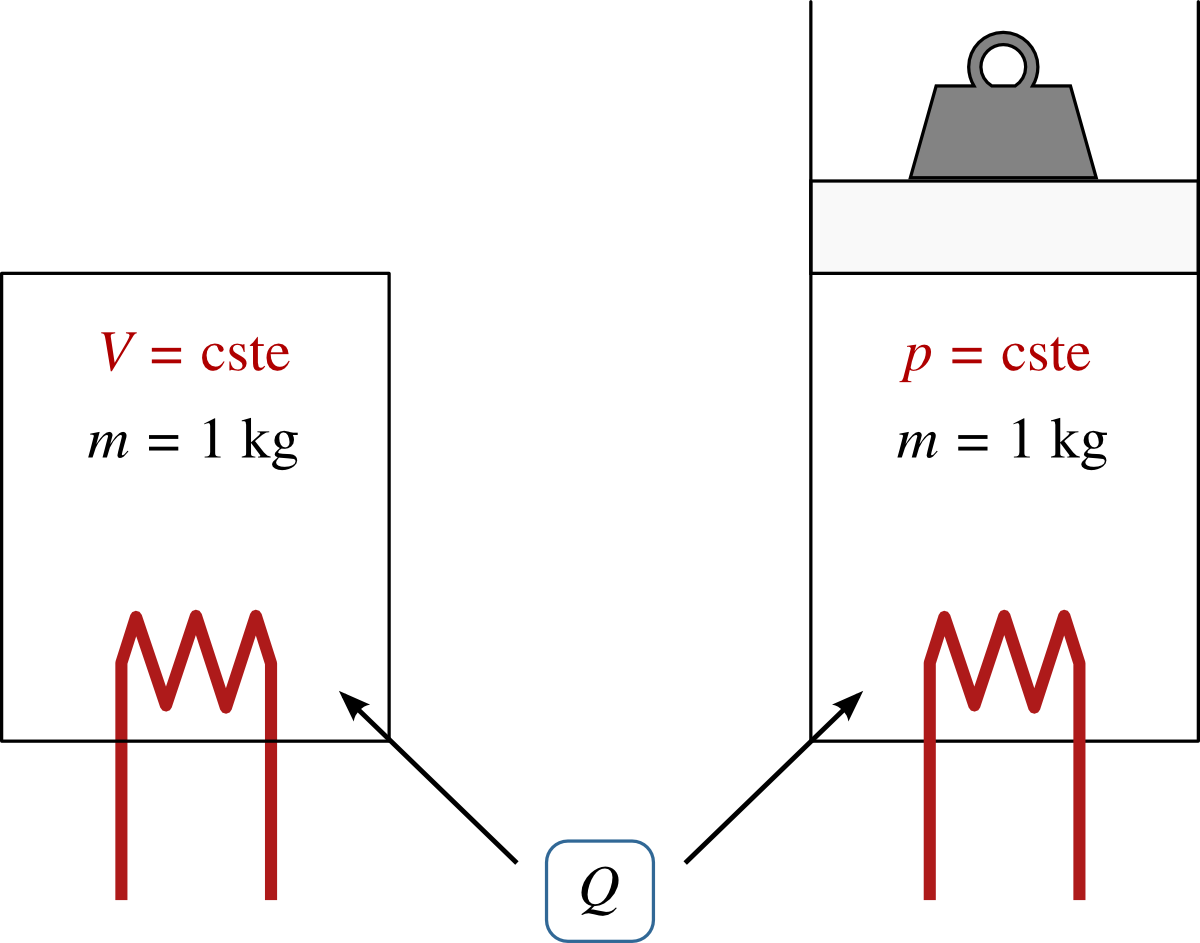
\includegraphics[width=10cm]{images/difference_capacites_calorifiques.png}
			\end{center}
			\caption{Deux quantités identiques de gaz reçoivent la même quantité de chaleur $Q$ . L’élévation de température sera plus faible à droite à cause du travail effectué sur le piston.}
			\label{fig_expérience_diff_chaleurs_massiques}
		\end{figure}

		Pourtant, deux valeurs particulières (\cref{fig_cp_et_cv}) suffisent pour décrire l’ensemble de ces comportements pour un gaz parfait :

		\begin{figure}
			\begin{center}
				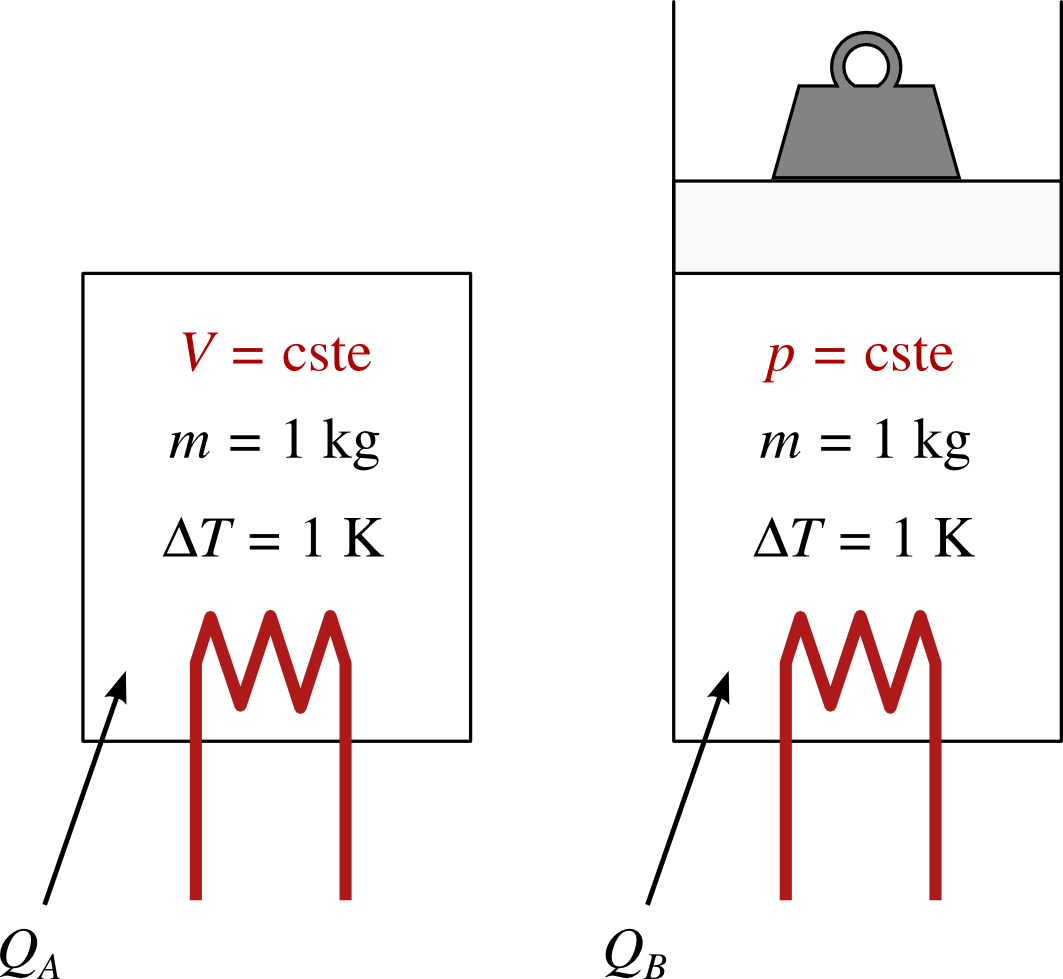
\includegraphics[width=9cm]{images/capacites_calorifiques.png}
			\end{center}
			\caption{Définitions des chaleurs massiques. À gauche, le volume est fixé et la capacité calorifique massique sera $c_v$. À droite, la pression est constante et la capacité sera $c_p$.}
			\label{fig_cp_et_cv}
		\end{figure}
		
		\begin{description}
			\item[la chaleur massique à volume constant :]$c_v$~, \dontbreakpage
			\item[la chaleur massique à pression constante :]$c_p$~.
		\end{description}


		Par définition, pour un gaz parfait, $c_v$ et $c_p$ sont indépendantes de la température. Pour les gaz réels, elles varient avec la température (\cref{fig_valeurs_de_cp_cv_gamma}), mais pour la plupart des applications une valeur moyenne peut être utilisée sans grande imprécision. Nous retiendrons les valeurs $c_{v  (air)} = \SI{718}{\joule\per\kilogram\per\kelvin}$ et $c_{p (air)} = \SI{1005}{\joule\per\kilogram\per\kelvin}$ pour l’air.

		\begin{figure}
			\begin{center}
				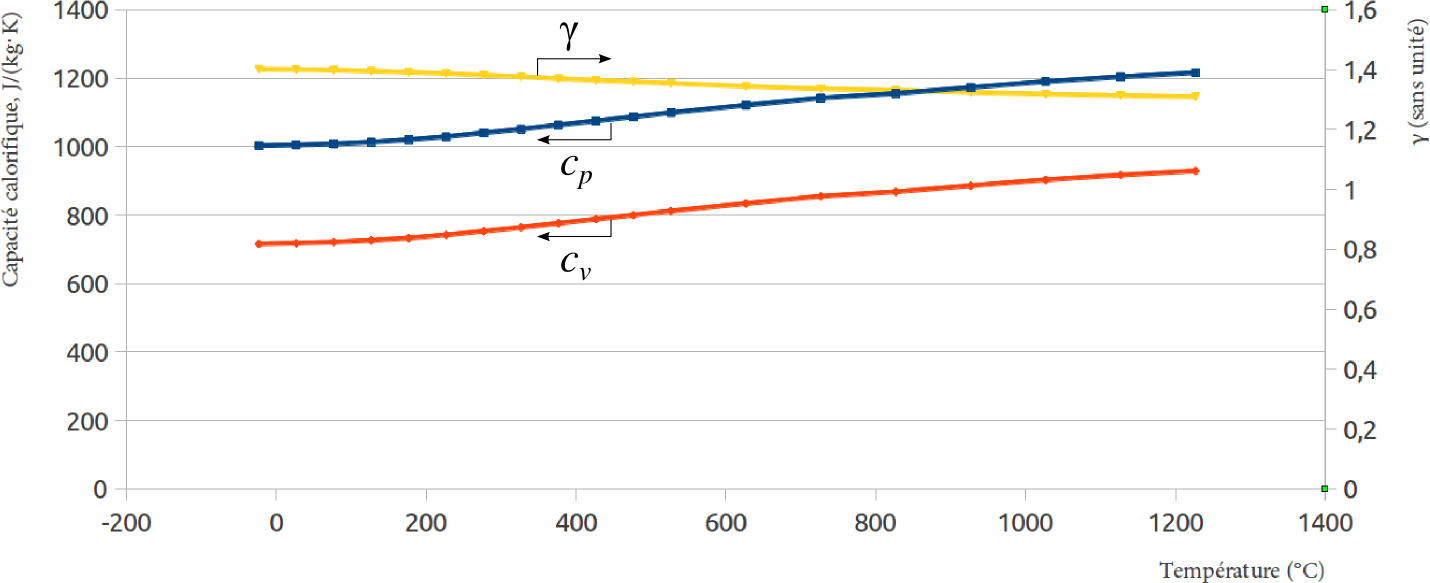
\includegraphics[width=15cm, inner]{images/cours4-img7.png}
			\end{center}
			\supercaption{Capacité calorifique de l’air en fonction de sa température. On note une variation sensible des valeurs dans la gamme de températures utilisée en ingénierie, que nous négligerons dans le cadre de notre étude de la thermodynamique.}%
				{Données issues du circulaire NBS 564 “Tables of Thermal Properties of Gases” (1955) jusqu’à~\SI{1000}{\kelvin}, calculées selon le modèle de B. G. Kyle in “Chemical and Process Thermodynamics” (1984) ensuite, et publiées par Israel Urieli (\href{http ://www.ohio.edu/mechanical/thermo/}{ohio.edu/mechanical/thermo/})}
		\label{fig_valeurs_de_cp_cv_gamma}
		\end{figure}




	\subsection{Différence des chaleurs massiques}

		Le grand nombre d’équations que nous abordons rend utile, mais pas indispensable, cette courte section. Pour l’ingénieur/e, il n’a d’autre intérêt que de permettre d’alléger l’écriture des relations de la section suivante.

		Observons les quantités d’énergie en jeu dans l’expérience décrite en \cref{fig_cp_et_cv}. Nous fournissons à chaque corps une quantité de chaleur différente pour obtenir la même variation de température. La différence entre les deux quantités de chaleur requises provient du fait que le gaz à pression constante (à droite) a fourni un travail pendant l’évolution.

		Quelle est la différence entre les chaleurs massiques de chacun des gaz ? Dans chacun des deux cas, nous avons $q_{1 \to 2} + w_{1 \to 2} = \Delta u$ (\ref{eq_premier_principe_sf_min}). Pour le corps A à gauche, comme aucun travail n’est effectué et que l’évolution est à volume constant, nous pouvons écrire :
			\begin{equation}
				\left\{
					\begin{array}{rl}
						q_\A 		& = c_v \ \Delta T \\
						\Delta u 			& = q_\A 
					\end{array} \right.
			\label{eq_sectionmathschiante_0}
			\end{equation}

		Pour le corps B à droite, comme la pression $p_\text{cste}$ est constante, nous pouvons écrire :


			\begin{equation}
				\left\{
					\begin{array}{rl}
						q_\B 		& = c_p \ \Delta T \\
						\Delta u 	& = q_\B + (-p_\text{cste} \ \Delta v)
					\end{array} \right.
			\label{eq_sectionmathschiante_1}
			\end{equation}


		En combinant les deux systèmes~\ref{eq_sectionmathschiante_0} et~\ref{eq_sectionmathschiante_1}%
			\footnote{En étant véritablement rigoureux, pour affirmer que $\Delta u_A$ et  $\Delta u_B$ sont égaux, il nous faudrait attendre l’\cref{eq_principe_de_joule} qui arrive à la section suivante.}%
		, nous obtenons

		\begin{equation}
			c_v \ \Delta T = c_p \ \Delta T - p_\text{cste} \ \Delta v
		\end{equation}

		qui stipule simplement que la différence entre les deux chaleurs fournies est retrouvée dans le travail fourni par le gaz de droite.

		Une brève manipulation amène :

		\begin{IEEEeqnarray}{rCl}
			(c_p - c_v) \Delta T 	& = & p_\text{cste} \ \Delta v	\nonumber \\
			(c_p - c_v) 				& = & \frac{pv_2 - pv_1}{\Delta T} = \frac{R T_2 - R T_1}{\Delta T_\B } = \frac{R \ \Delta T}{\Delta T}	\nonumber \\
			c_p - c_v 					& = & R
		\label{eq_sectionmathschiante_2}
		\end{IEEEeqnarray}

		Cette expression a pour seul intérêt de nous permettre de simplifier l’\cref{eq_h_fonction_de_T} que nous allons écrire plus bas.


		\subsection{Quotient des chaleurs massiques}

		Le ratio des chaleurs massiques à pression et à volume constants est nommé $\gamma $. Ainsi :
		\begin{equation}
			\gamma  \equiv  \frac{c_p}{c_v}
			\label{def_gamma}
		\end{equation}

		En retournant à la \cref{fig_cp_et_cv} il apparaît rapidement que $c_p$ doit être supérieur à $c_v$ ; ainsi $\gamma$ est toujours supérieur à~1. La valeur de $\gamma$ est d’environ \num{1,4} pour l’air.
		
		

\section{Énergie et température}

	\subsection{La loi de Joule}
	\label{ch_principe_de_joule}

		Alors qu’il se pose des questions sur la nature de la chaleur et du travail%
			\footnote{Ces questions surviennent au cours d’une série de travaux soignés qui mèneront à la première expression formelle du premier principe de la thermodynamique, et à la fin de la théorie du \textit{calorique} selon laquelle la chaleur était un fluide très peu dense et invisible. Ils vaudront à son nom de famille l’utilisation que l’on sait aujourd’hui.}%
		, \wf{James Prescott Joule} étudie dans les années 1840 la relation entre l’énergie interne d’un gaz et sa température.

		Lors d’une de ses expériences les plus remarquables, il cherche à faire varier la pression et le volume d’un gaz \textit{sans lui transférer de chaleur ou de travail}. Pour cela, il laisse un gaz comprimé se détendre dans un second récipient vide (\cref{fig_detente_joule}), et mesure le flux de chaleur vers le gaz. Le travail effectué est nul%
		\footnote{Le travail effectué est nul car l’évolution est parfaitement irréversible : aucune surface n’a été déplacée.}%
		, et… il ne se passe rien ! Joule ne mesure ni flux de chaleur, ni variation de température.

		\begin{figure}
			\begin{center}
				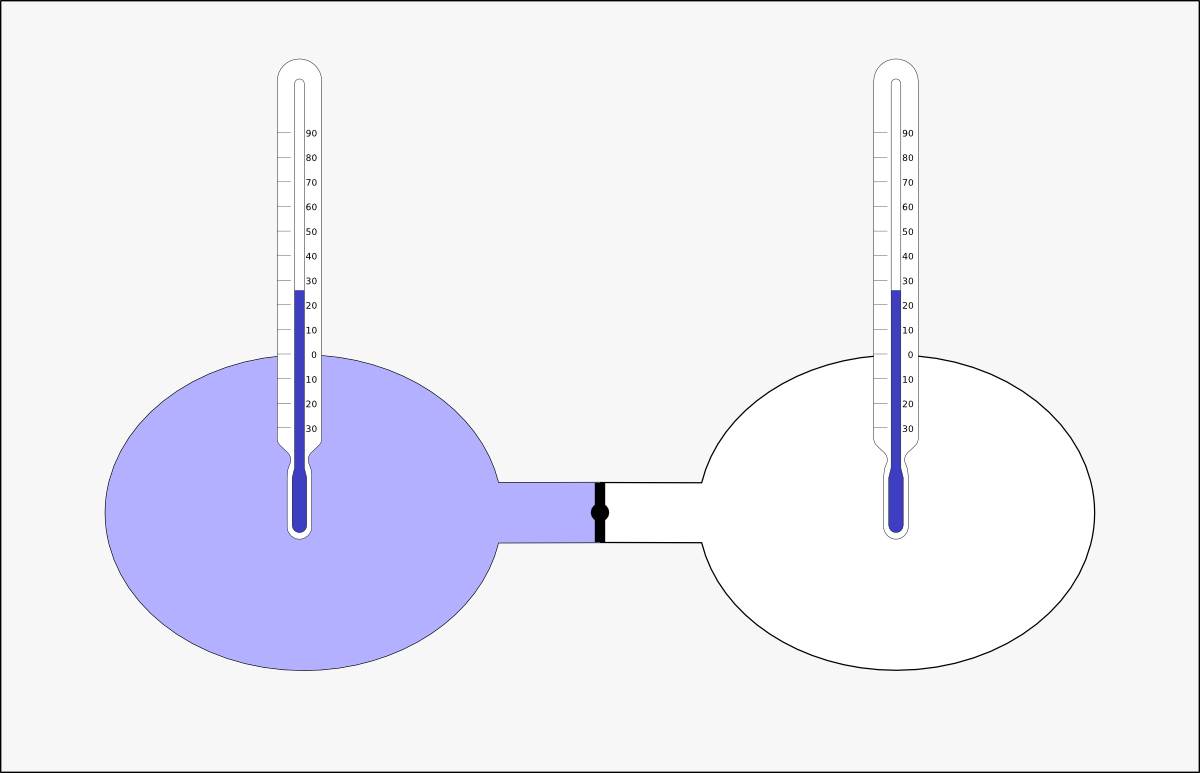
\includegraphics[width=9cm]{images/cours4-img8.png}
			\end{center}
			\supercaption{La détente de Joule, parfois appelée \wfd{D\%C3\%A9tente de Joule-Gay-Lussac}{détente de Joule et Gay-Lussac}.\\			
		Un gaz est initialement prisonnier d’un réservoir à gauche ; on le laisse se détendre en ouvrant la vanne (au centre) qui le sépare d’un réservoir entièrement vide à droite.\\		
		Joule s’intéresse aux variations de température mesurées dans chaque réservoir. Plus les propriétés du gaz rapprochent son comportement du modèle des gaz parfaits (\S\ref{ch_pas_gaz_parfait}), et plus les variations de température qu’il mesure sont faibles, jusqu’à devenir indétectables pour certains gaz simples à haute température).\par}{}
			\label{fig_detente_joule}
		\end{figure}

		Joule effectue une multitude d’expériences différentes au cours desquelles il observe que quel que soit le travail fourni, la relation entre énergie interne (qui ne varie qu’avec travail et chaleur) et température reste sensiblement la même --\ et il suggère que pour un gaz parfait, elle reste toujours identique.

		Ce postulat est connu sous le nom de \vocab{principe de Joule} et est posé comme vrai pour tout gaz parfait. On peut le résumer ainsi :

		\begin{trucimportant}
			La température d’un gaz parfait ne varie qu’avec son énergie interne.
		\end{trucimportant}

		Mathématiquement, nous pouvons l’écrire ainsi :
		\begin{equation}
			u = f(T)
		\end{equation}

		La fonction $f$ peut être évaluée avec une expérience dans laquelle la variation de~$u$ est quantifiée. Par exemple, lors d’une évolution à volume constant $q = \Delta u$ et $q = c_v \ \Delta T$. On peut ainsi affirmer que la fonction $f$ est une simple relation de proportionnalité. L’énergie interne pouvant être arbitrairement posée comme nulle à température nulle ($u = \SI{0}{\joule\per\kilogram}$ lorsque $T = \SI{0}{\kelvin}$), on obtient :
		\begin{equation}
			u = c_v \ T
			\label{eq_principe_de_joule}
		\end{equation}

		\begin{equationterms}
			\item pour tout gaz parfait,
			\item quelle que soit l’évolution (réversible ou non),
			\item où \tab $u$ \tab est l’énergie interne spécifique (\si{\joule\per\kilogram}) ;
			\item \tab $T$ \tab est la température (\si{\kelvin}) ;
			\item et \tab $c_v$ \tab est la capacité calorifique massique à volume constant (\si{\joule\per\kilogram\per\kelvin}).
		\end{equationterms}

		Pour une masse $m$ de gaz parfait, on a bien sûr :
		\begin{equation}
			U = m \ c_v \ T
		\end{equation}

		Tant que notre fluide se comporte comme un gaz parfait, cette relation~\ref{eq_principe_de_joule} reste vraie. Elle fonctionne pendant toute évolution, réversible ou non, et quelles que soient les contraintes de volume, de pression ou température.

		Par contre, il faut bien noter que cette \cref{eq_principe_de_joule}, qui découle du principe de Joule, n’est pas du tout valable dans le cas des liquides et vapeurs. On peut, par exemple, ajouter de l’énergie à une masse d’eau bouillante, sans que sa température n’augmente. Nous étudierons les liquides et vapeurs dans le \courscinqshort.



	\subsection{Enthalpie d’un gaz parfait}

		Parce que nous venons de lier l’énergie interne $u$ à la température, et que le produit $p v$ dépend lui aussi de la température, nous pouvons désormais facilement exprimer l’enthalpie $h$ d’un gaz parfait en fonction de la température uniquement.

		En effet, nous avons $h \equiv  u + p v$ (\ref{def_enthalpie}) ; avec une rapide insertion des équations~\ref{eq_pv=RT} et~\ref{eq_principe_de_joule} il vient, pour tout gaz parfait :
			\begin{equation}
				h = u + p v = c_v T + R T = (c_v + R) \ T
				\label{eq_h_fonction_de_T}
			\end{equation}

		Avec l’\cref{eq_sectionmathschiante_2} que nous avons développée plus haut, nous pouvons simplifier cette expression pour obtenir :
			\begin{equation}
				h = c_p \ T
				\label{eq_h=cpT}
			\end{equation}

			\begin{equationterms}
				\item Pour tout gaz parfait,
				\item quelle que soit l’évolution (réversible ou non),
				\item où \tab $h$ \tab est l’enthalpie spécifique (\si{\joule\per\kilogram}) ;
				\item \tab $T$ \tab est la température (\si{\kelvin}) ;
				\item et \tab $c_p$ \tab est la capacité calorifique massique à pression constante (\si{\joule\per\kilogram\per\kelvin}).
			\end{equationterms}


	\subsection{Interlude : Que retenir du gaz parfait jusqu’ici ?}

		Le gaz parfait est un modèle pour quantifier la température d’un gaz. Selon ce modèle, les trois principales formes d’énergie que nous avons utilisées jusqu’à présent —~l’énergie interne~$u$, l’enthalpie spécifique~$h$ et le terme~$p v$~— sont directement proportionnelles à la température~$T$ :

		\begin{IEEEeqnarray*}{rClC}
			u 	& = & c_v T 	& \qquad (\si{\joule\per\kilogram})	\\
			h 	& = & c_p T	& \qquad (\si{\joule\per\kilogram}) 	\\
			p v 	& = & R T 	& \qquad (\si{\joule\per\kilogram})
		\end{IEEEeqnarray*}

		Si l’on contrôle la température d’un gaz (par exemple avec un transfert de chaleur), alors on affecte directement et simultanément ces trois formes d’énergie.




\section{Transformations élémentaires réversibles}
\label{ch_gp_evolutions_elementaires}

	Nous nous proposons ici de calculer les propriétés d’un gaz parfait, ainsi que les transferts d’énergie en jeu, lorsque l’on le comprime ou détend selon des contraintes entièrement arbitraires de volume, pression ou température.


	\subsection{À quoi sert cette section de chapitre ?}
	\label{ch_gp_evolutions_elementaires_aquoisert}

		Les évolutions de gaz que nous étudions ici sont très hypothétiques et pas nécessairement passionnantes, mais elles méritent l’attention de l’étudiant/e pour deux raisons :

		\begin{enumerate}
			\item Le comportement d’un gaz, même avec le modèle du gaz parfait, est intrinsèquement complexe. Ces évolutions élémentaires font figure de gymnastique et permettent d’apprendre à le décrire étape par étape ;
			\item Ces évolutions élémentaires sont des outils conceptuels que nous assemblerons plus tard, d’abord pour quantifier les limites théoriques des machines (au \coursseptshort), et enfin pour décrire le comportement des gaz à l’intérieur des machines réelles (au \coursdixshort).
		\end{enumerate}


	\subsection{Évolutions à pression constante}
	\label{ch_gp_isobares}

		Il est possible de chauffer ou refroidir un gaz en maintenant sa pression constante (\cref{fig_gp_pression_constante}). Une évolution à pression constante est parfois dite \vocab{isobare}. Pour générer une telle transformation, nous pouvons :
		
		\begin{itemize}
			\item avec un système fermé, chauffer ou refroidir le gaz en maintenant une force constante sur les parois ;
			\item avec un système ouvert, chauffer ou refroidir le gaz en le laissant simplement s’écouler dans un conduit, sans pièce mobile. C’est le cas par exemple dans la chambre de combustion d’un turboréacteur.
		\end{itemize}

		\begin{figure}
			\begin{center}
				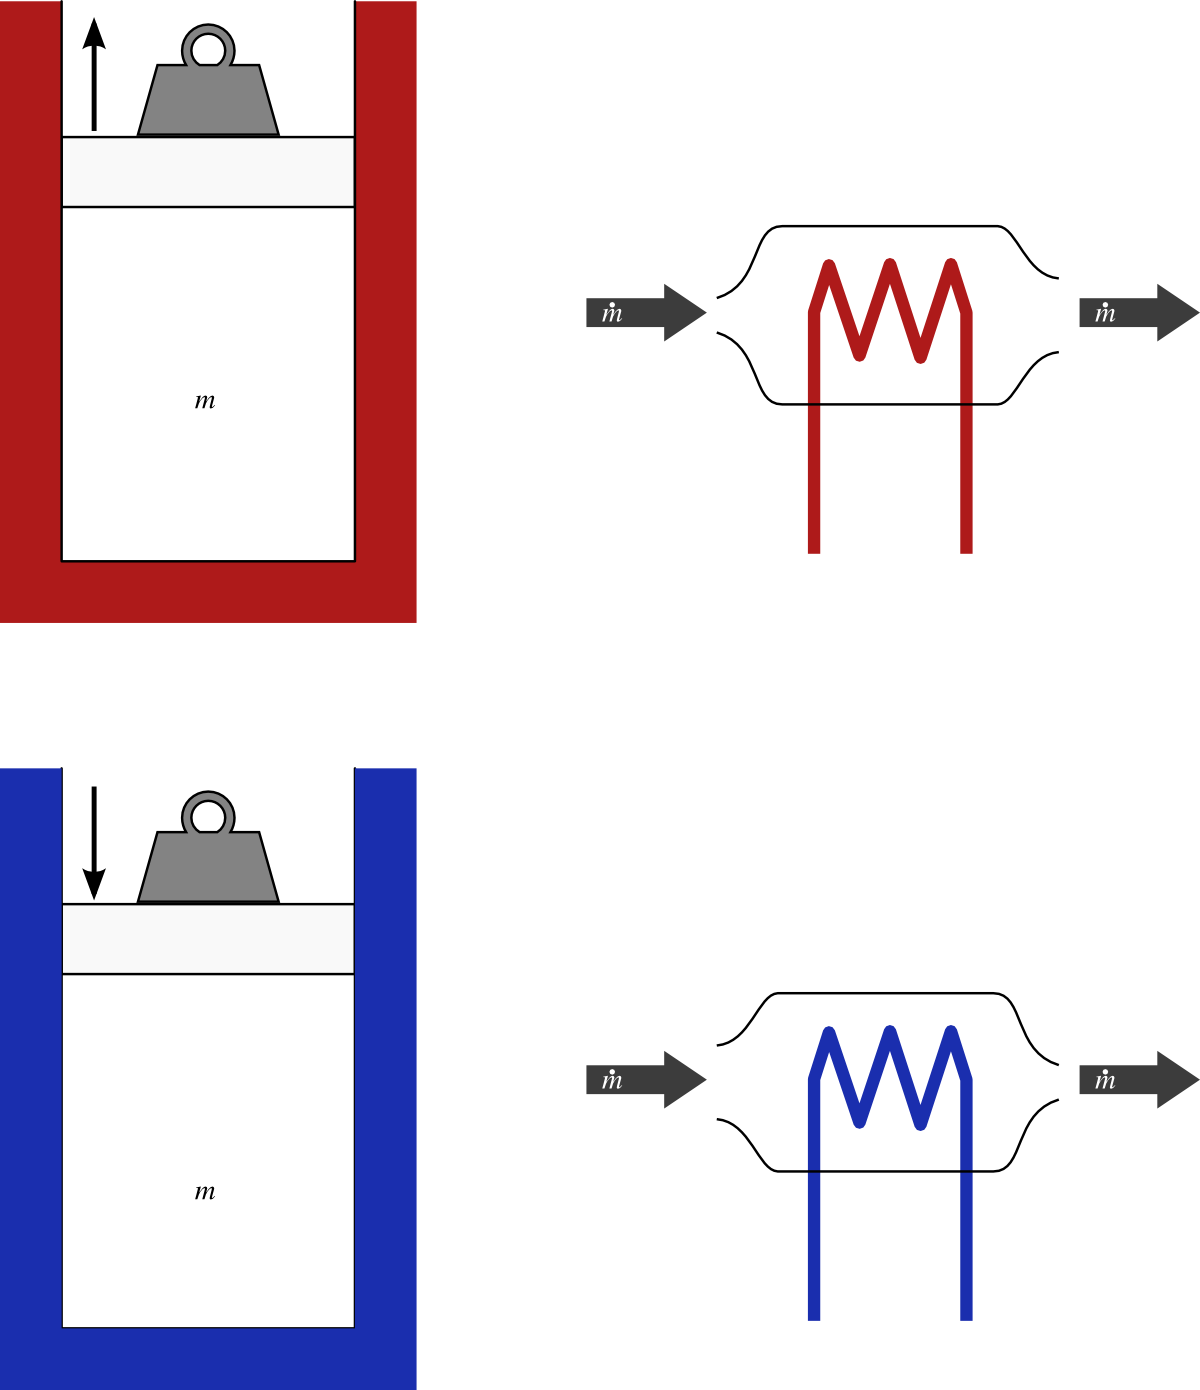
\includegraphics[width=10cm]{images/pression_constante.png}
			\end{center}
			\caption{Évolution à pression constante (isobare) d’un gaz parfait. En système fermé (à gauche), le piston exerce une force constante tout au long de l’évolution. En système ouvert (à droite), aucun travail n’est effectué.}
			\label{fig_gp_pression_constante}
		\end{figure}
		
		\begin{figure}
			\begin{center}
				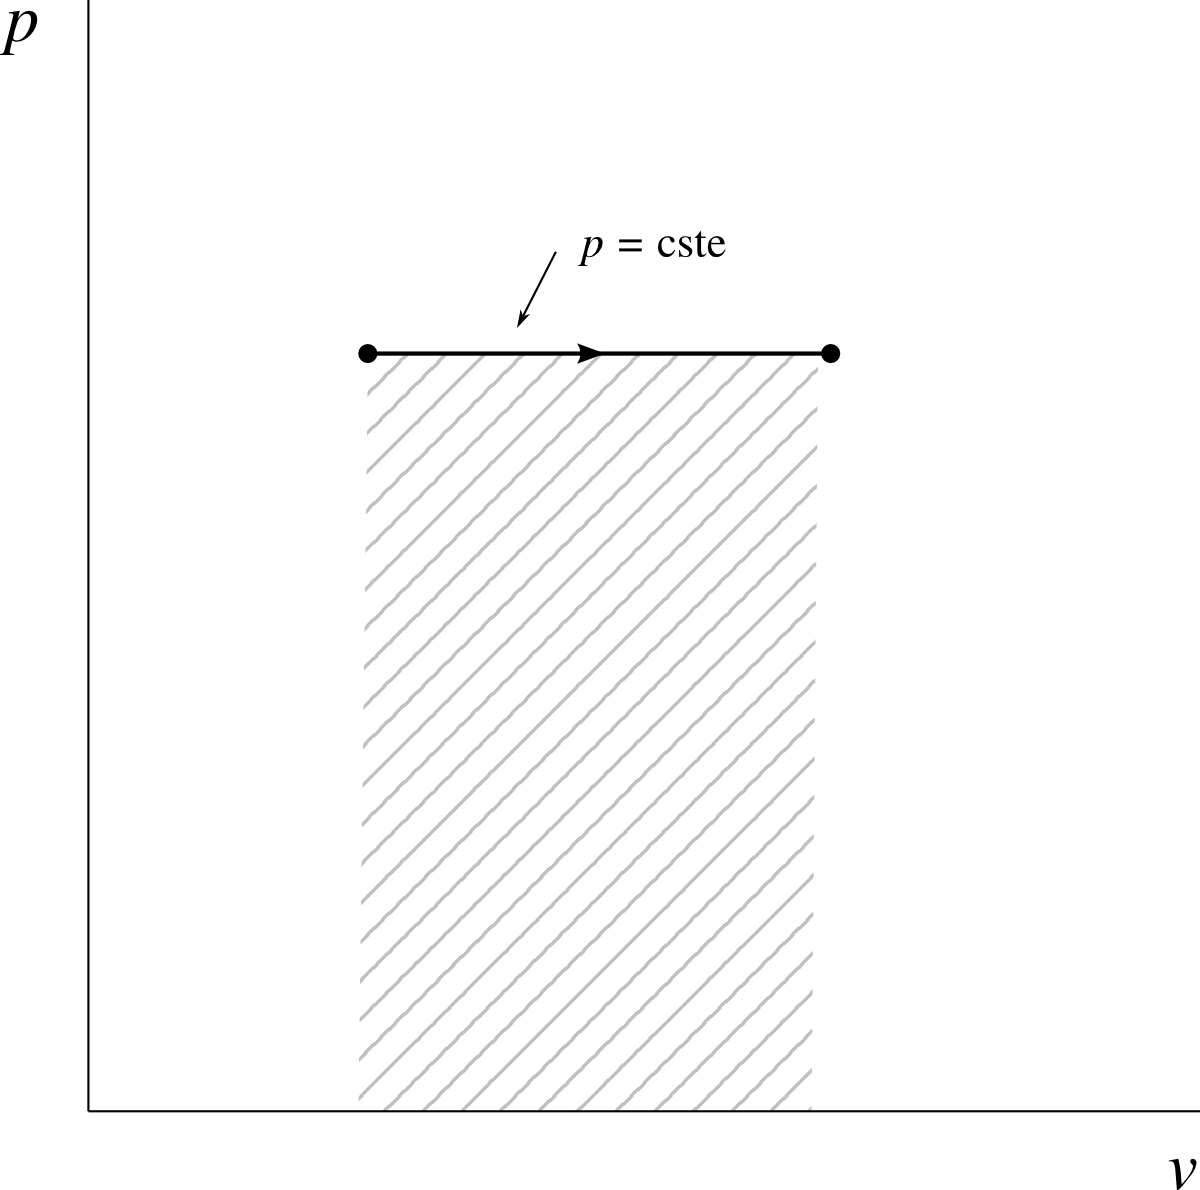
\includegraphics[width=8cm]{images/pv_isobare.png}
			\end{center}
			\caption{Réchauffement à pression constante d’un gaz parfait, représenté sur un diagramme pression-volume.}
			\label{fig_gp_pression_constante_pv}
		\end{figure}		

		Lorsque la pression est constante, les propriétés du gaz varient selon la relation
		
		\begin{equation}
			\frac{T}{v} = \text{constante}
		\end{equation}
		
		
		En système fermé, nous avons $q_{1\to2} + w_{1\to2} = \Delta u$, et, si l’évolution est réversible, la chaleur et le travail peuvent être facilement reliés à la température :
		
		\begin{IEEEeqnarray}{rCl}
			w_{1\to2} 	& = & - \int _1^2 p \diff v  = -p_\text{cste} \int _1^2 \diff v = -p_\text{cste} \ \Delta v	\nonumber \\
			w_{1 \to 2} 	& = & - R \ \Delta T
		\end{IEEEeqnarray}
		\begin{equationterms}
			\item lors d’une évolution réversible à pression constante $p_\text{cste}$, en système fermé.
		\end{equationterms}

		On remarque que le travail est de signe opposé à la variation de température. 
		
		La chaleur peut être quantifiée aisément :
		
		\begin{IEEEeqnarray}{rCl}
			q_{1\to2} 	& = & \Delta u - w_{1\to2} = \Delta u + p_\text{cste} \ \Delta v = \Delta h \nonumber \\
			q_{1 \to 2} 	& = & c_p \ \Delta T
		\end{IEEEeqnarray}
		\begin{equationterms}
			\item lors d’une évolution réversible à pression constante, en système fermé.
		\end{equationterms}

		
		Lorsque l’évolution se fait en système ouvert, nous avons $q_{1\to2} + w_{1\to2} = \Delta h$, et, si l’évolution est réversible, la chaleur et le travail se quantifient sans peine :
		
		\begin{IEEEeqnarray}{rCl}
			w_{1\to2} 	& = & \int _1^2 v \diff p \nonumber \\
			w_{1\to2} 	& = & 0
		\end{IEEEeqnarray}
		\begin{equationterms}
			\item lors d’une évolution réversible à pression constante, en système ouvert.
		\end{equationterms}

		Le travail est bien sûr nul, puisqu’aucune pièce mobile n’est présente pour extraire de l’énergie mécanique du gaz.

		La chaleur est alors responsable de l’entièreté de la variation de température :
		
		\begin{IEEEeqnarray}{rCl}
			q_{1\to2} 	& = & \Delta h - w_{1\to2} = \Delta h \nonumber \\
			q_{1 \to 2} 	& = & c_p \ \Delta T
		\end{IEEEeqnarray}
		\begin{equationterms}
			\item lors d’une évolution réversible à pression constante, en système ouvert.
		\end{equationterms}



	\subsection{Évolutions à volume constant}
	\label{ch_gp_isochores}

		Il est possible de chauffer ou refroidir un gaz en maintenant son volume constant (\cref{fig_gp_volume_constant}). Une évolution à volume constant est parfois dite \vocab{isochore}.
			
		\begin{itemize}
			\item Avec un système fermé, nous pouvons chauffer ou refroidir un gaz dans un réservoir fixe et fermé. C’est le cas par exemple pendant la phase de combustion («~explosion~») dans un moteur à essence.
			\item Avec un système ouvert, la manipulation est plus complexe. Nous devons compresser le gaz pendant qu’on le réchauffe pour éviter que son volume n’augmente ; À l’inverse, pendant un refroidissement, il faut le détendre pour éviter que son volume ne baisse. Cette manipulation n’a pas d’application pratique courante.
		\end{itemize}	
		
		\begin{figure}
			\begin{center}
				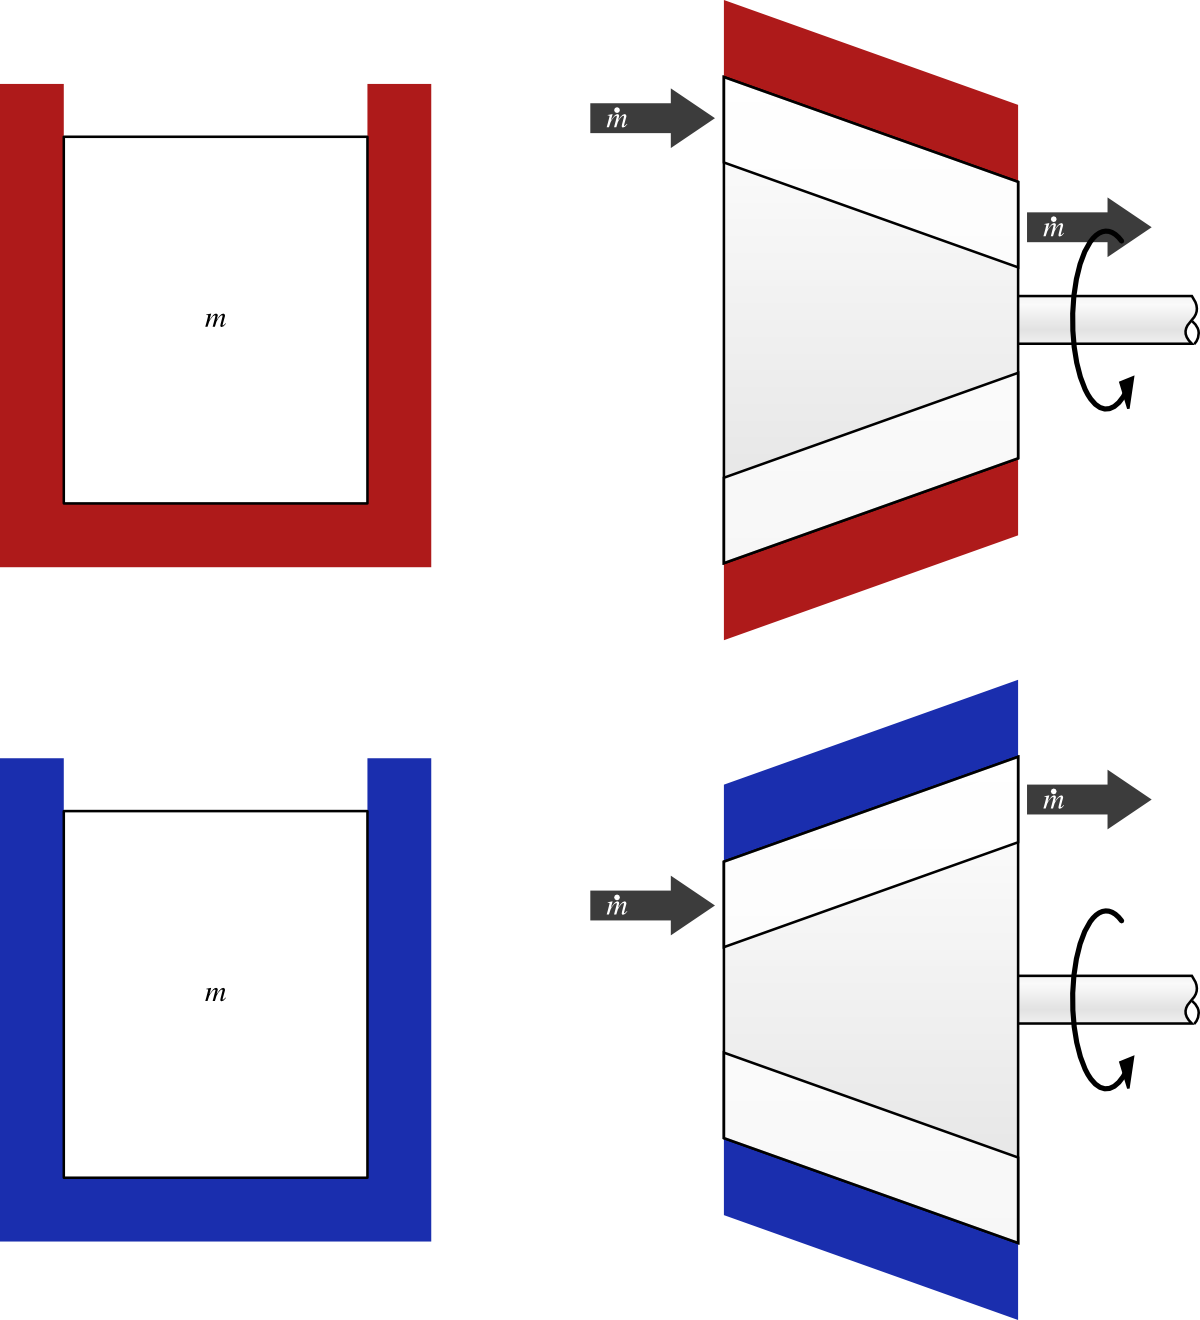
\includegraphics[width=10cm]{images/volume_constant.png}
			\end{center}
			\caption{Évolution à volume constant (isochore) d’un gaz parfait. En système fermé (à gauche), le volume est bloqué et aucun travail n’est effectué. En système ouvert (à droite), on doit comprimer le gaz pendant qu’on le chauffe et le détendre pendant qu’on le refroidit, pour pouvoir maintenir le volume spécifique constant.}
			\label{fig_gp_volume_constant}
		\end{figure}
		
		\begin{figure}
			\begin{center}
				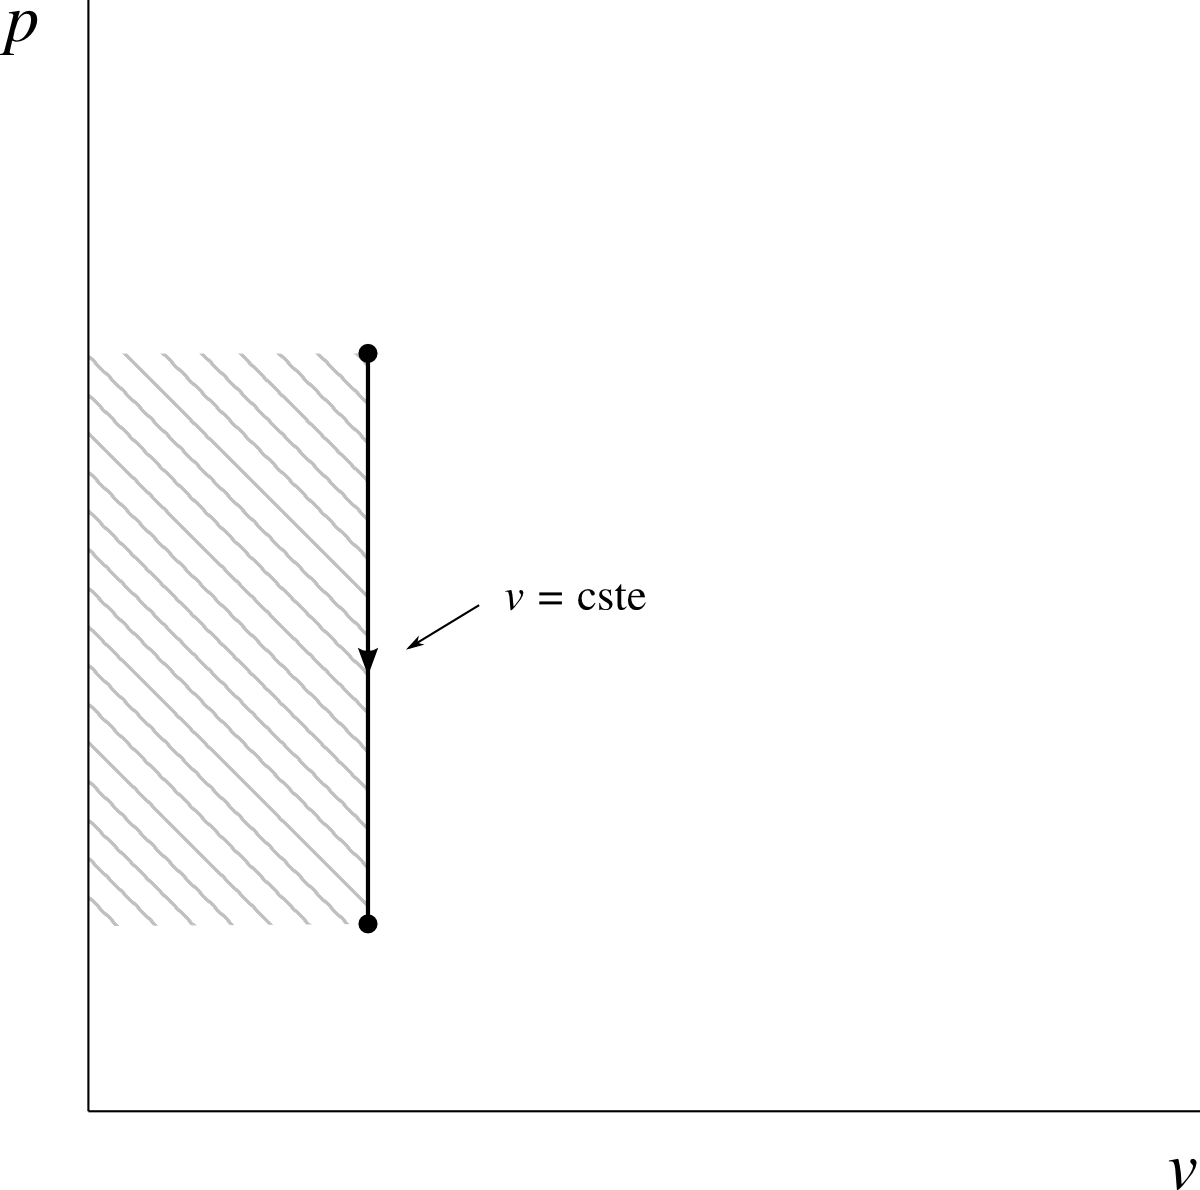
\includegraphics[width=8cm]{images/pv_isochore.png}
			\end{center}
			\caption{Refroidissement à volume constant d’un gaz parfait, représenté sur un diagramme pression-volume.}
			\label{fig_gp_volume_constant_pv}
		\end{figure}		

		Lorsque le volume spécifique d’un gaz parfait est constant, ses propriétés varient selon la relation 
		
		\begin{equation}
			\frac{T}{p} = \text{constante}
		\end{equation}
		
		En système fermé, nous avons $q_{1\to2} + w_{1\to2} = \Delta u$, et, si l’évolution est réversible, la chaleur et le travail peuvent être facilement reliés à la température.

		Le volume ne variant pas, le travail est bien sûr nul :
		
		\begin{IEEEeqnarray}{rCl}
			w_{1\to2} 	& = & - \int _1^2 p \diff v	\nonumber \\
			w_{1\to2} 	& = & 0
		\end{IEEEeqnarray}
		\begin{equationterms}
			\item lors d’une évolution réversible à volume constant, en système fermé.
		\end{equationterms}

		La chaleur peut être quantifiée aisément :
		
		\begin{IEEEeqnarray}{rCl}
			q_{1\to2} 	& = & \Delta u - w_{1\to2} = \Delta u \nonumber \\
			q_{1\to2} 	& = & c_v \ \Delta T
		\end{IEEEeqnarray}
		\begin{equationterms}
			\item lors d’une évolution réversible à volume constant, en système fermé.
		\end{equationterms}

		
		Lorsque l’évolution se fait en système ouvert, nous avons $q_{1\to2} + w_{1\to2} = \Delta h$, et, si l’évolution est réversible, la chaleur et le travail peuvent être quantifiés, bien qu’avec un peu plus de difficulté :
		
		\begin{IEEEeqnarray}{rCl}
			w_{1\to2} 	& = & \int _1^2 v \diff p = v_\text{cste} \int_1^2 \diff p = v_\text{cste} \int_1^2 \frac{R}{v_\text{cste}} \diff T = R \int_1^2 \diff T  \nonumber \\
			w_{1\to2} 	& = & R \ \Delta T
		\end{IEEEeqnarray}
		\begin{equationterms}
			\item lors d’une évolution réversible à volume constant, en système ouvert.
		\end{equationterms}

		On peut alors quantifier facilement la chaleur à fournir :
		
		\begin{IEEEeqnarray}{rCl}
			q_{1\to2} 	& = & \Delta h - w_{1\to2} = c_p \ \Delta T - R \ \Delta T \nonumber \\
			q_{1\to2} 	& = & c_v \ \Delta T
		\end{IEEEeqnarray}
		\begin{equationterms}
			\item lors d’une évolution réversible à volume constant, en système ouvert.
		\end{equationterms}


	\subsection{Évolutions à température constante}
	\label{ch_gp_isothermes}
	
		Il est possible de chauffer ou refroidir un gaz en maintenant sa température constante (\cref{fig_gp_température_constante}). Une évolution à température constante est parfois dite \vocab{isotherme}. 
		
		\begin{figure}
			\begin{center}
				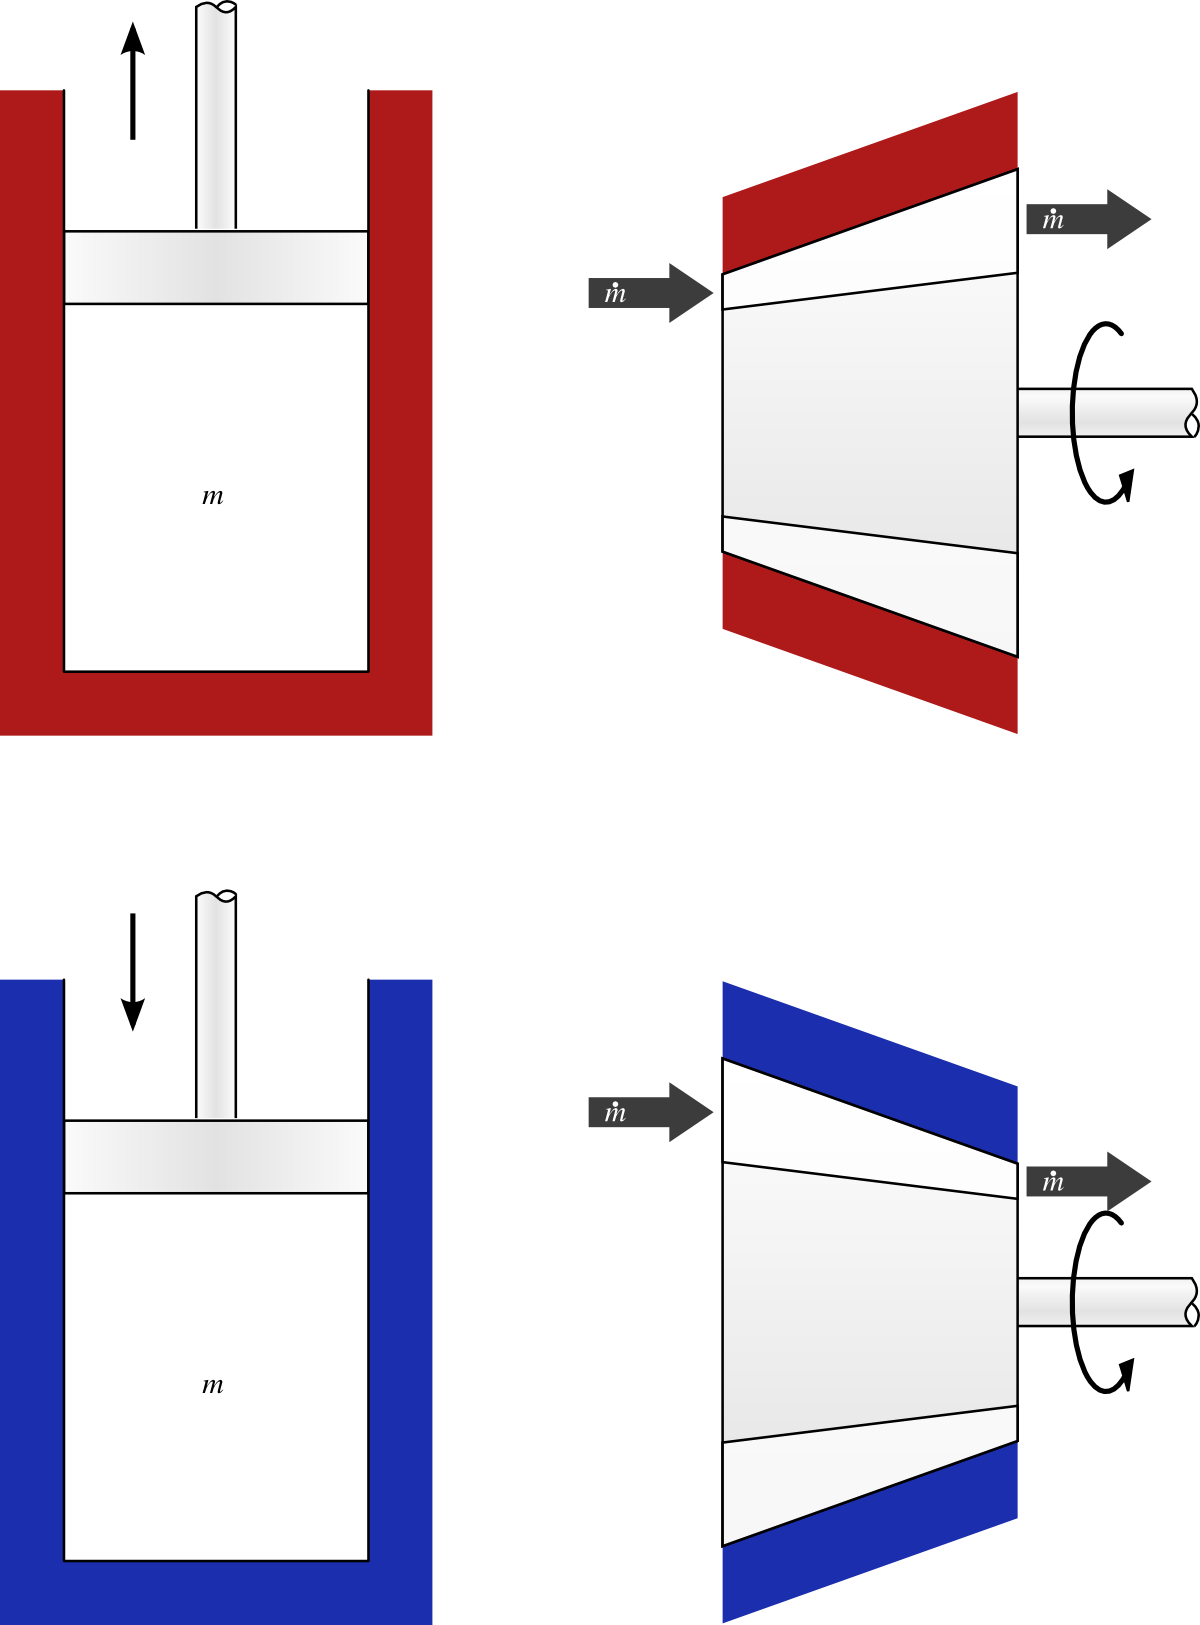
\includegraphics[width=10cm]{images/temperature_constante.png}
			\end{center}
			\caption{Évolution à température constante (isotherme) d’un gaz parfait. En système fermé (à gauche), on laisse travailler le gaz sur un piston pendant qu’on le chauffe, et à l’inverse, on lui fournit du travail lorsqu’on le refroidit. En système ouvert (à droite), les mêmes manipulations sont effectuées en flux continu.}
			\label{fig_gp_température_constante}
		\end{figure}
		
		\begin{figure}
			\begin{center}
				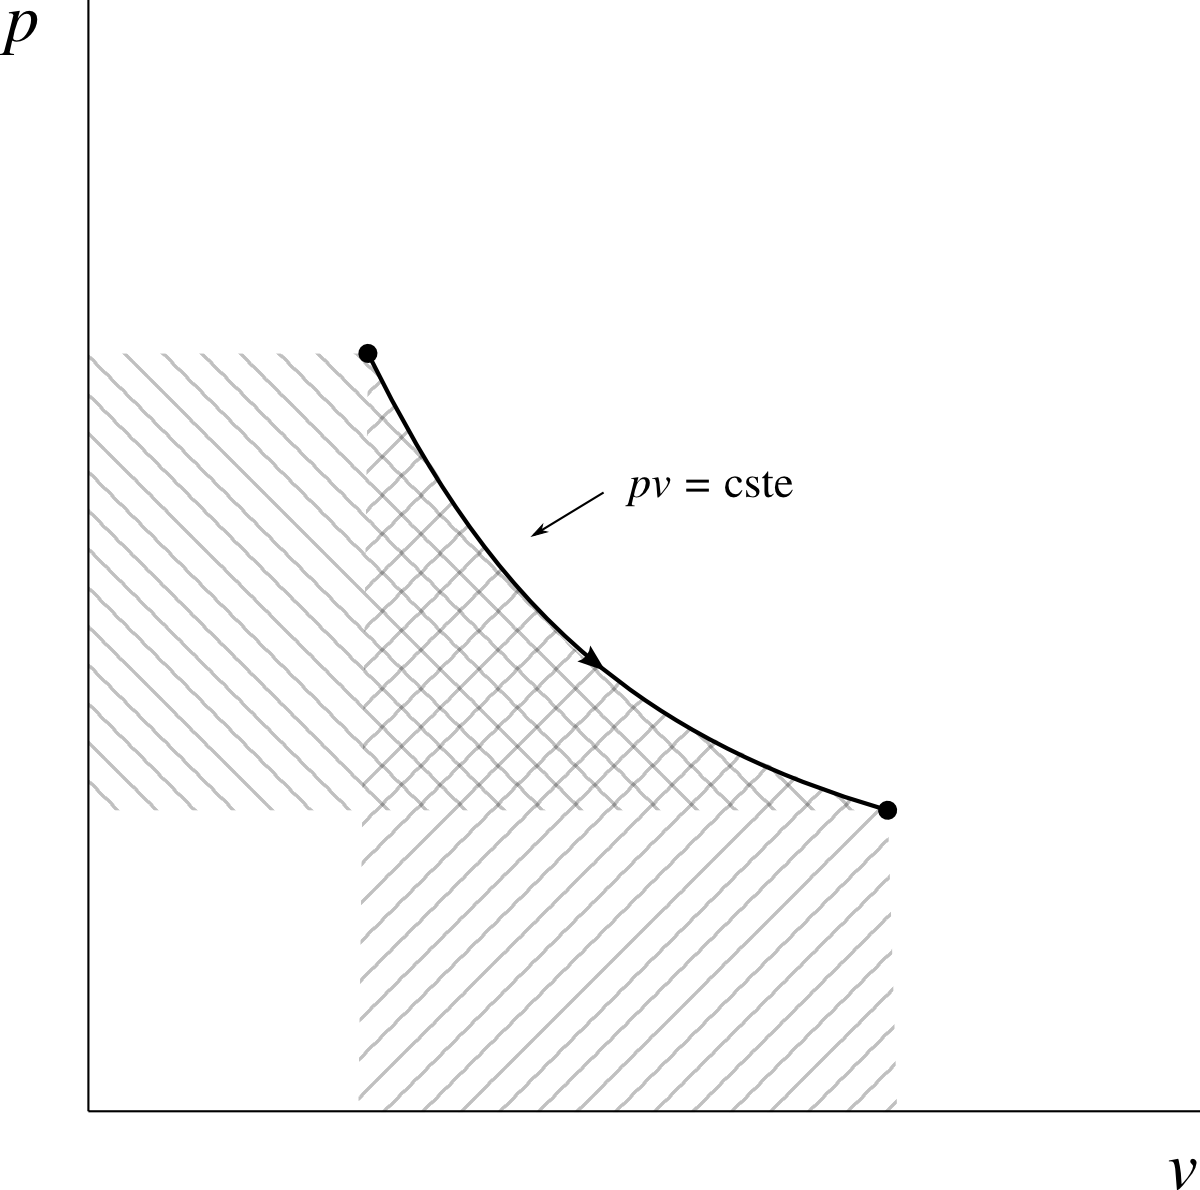
\includegraphics[width=8cm]{images/pv_isotherme.png}
			\end{center}
			\caption{Détente (réchauffement) à température constante d’un gaz parfait, représenté sur un diagramme pression-volume.}
			\label{fig_gp_température_constante_pv}
		\end{figure}		

		Pour un gaz parfait, une évolution à température constante se fait toujours à énergie constante. Pour chaque joule de chaleur que l’on fournit au gaz, il faut lui prendre un joule sous forme de travail ; inversement chaque prélèvement de chaleur doit être compensé par un apport égal de travail.
		
		En pratique, cette complexité fait que les transferts de chaleur isothermes sont rarement utilisés dans l’industrie. Ils revêtent par contre une importance théorique capitale, que nous étudierons au \courssept.
		
		Lorsque la température d’un gaz parfait reste constante, ses propriétés varient selon la relation 
		
		\begin{equation}
			p \ v = \text{constante}
			\label{eq_pvconstante}
		\end{equation}
		

		En système fermé, nous avons $q_{1\to2} + w_{1\to2} = \Delta u$, et, si l’évolution est réversible, la chaleur et le travail peuvent être reliés aux propriétés du gaz, non sans une certaine difficulté.

		\begin{IEEEeqnarray}{rCl}
			w_{1\to2} 	& = & - \int _1^2 p \diff v = - \int \frac{R T_\text{cste}}{v} \diff v = - R T_\text{cste} \int_1^2 \frac{1}{v} \diff v = - R T_\text{cste} [\ln v]_{v_1}^{v_2} \nonumber \\
			w_{1\to2} 	& = & R T_\text{cste} \ln \left(\frac{v_1}{v_2}\right)
			\label{eq_travail_température_constante}
		\end{IEEEeqnarray}
		\begin{equationterms}
			\item lors d’une évolution réversible à température constante, en système fermé.
		\end{equationterms}

		On peut aussi exprimer le travail en fonction de la pression, puisqu’avec l’\cref{eq_pvconstante} on~a :
		
		\begin{equation*}
			\frac{v_1}{v_2} = \frac{p_2}{p_1}
		\end{equation*}
		
		ainsi :
		
		\begin{equation}
			w_{1\to2} 	 = R T_\text{cste} \ln \left(\frac{p_2}{p_1}\right)
			\label{eq_gp_travail_isotherme_sf}
		\end{equation}
		\begin{equationterms}
			\item lors d’une évolution réversible à température constante, en système fermé.
		\end{equationterms}

		La chaleur peut être quantifiée aisément. En effet, l’énergie interne ne varie pas :
		
		\begin{IEEEeqnarray}{rCl}
			q_{1\to2} 	& = & \Delta u - w_{1\to2} = 0 - w_{1\to2} \nonumber \\
			q_{1\to2} 	& = & -w_{1\to2}
			\label{eq_gp_chaleur_isotherme_sf}
		\end{IEEEeqnarray}
		\begin{equationterms}
			\item lors d’une évolution réversible à température constante, en système fermé.
		\end{equationterms}

		
		Lorsque l’évolution se fait en système ouvert, nous avons $q_{1\to2} + w_{1\to2} = \Delta h$, et, si l’évolution est réversible, la chaleur et le travail peuvent être quantifiés de la même façon :
		
		\begin{IEEEeqnarray}{rCl}
			w_{1\to2} 	& = & \int _1^2 v \diff p = \int_1^2 \frac{R T_\text{cste}}{p} \diff p = R T_\text{cste} \int_1^2 \frac{1}{p} \diff p = R T_\text{cste} [\ln v]_{p_1}^{p_2} \nonumber \\
			w_{1\to2} 	& = & R T_\text{cste} \ln \left(\frac{p_2}{p_1}\right) = R T_\text{cste} \ln \left(\frac{v_1}{v_2}\right) \label{eq_travail_température_constante_rep}
		\end{IEEEeqnarray}
		\begin{equationterms}
			\item lors d’une évolution réversible à température constante, en système ouvert.
		\end{equationterms}
		
		Cette relation, identique à l’\cref{eq_travail_température_constante}, n’aura pas surpris l’étudiant/e perspicace, puisque la relation $p v = \text{cste}$ assure que pour deux points donnés en \cref{fig_gp_température_constante_pv}, l’aire sous la courbe soit toujours égale à l’aire à gauche de la courbe.

		La chaleur à fournir se quantifie bien sûr sans peine :
		
		\begin{IEEEeqnarray}{rCl}
			q_{1\to2} 	& = & \Delta h - w_{1\to2} = 0 - w_{1\to2} \nonumber \\
			q_{1\to2} 	& = & - w_{1\to2}
		\end{IEEEeqnarray}
		\begin{equationterms}
			\item lors d’une évolution réversible à température constante, en système ouvert.
		\end{equationterms}




	\subsection{Évolutions adiabatiques réversibles}
	\label{ch_gp_isentropiques}

		Une évolution \vocab{adiabatique} est une évolution au cours de laquelle il n’y a aucun échange de chaleur (\cref{fig_gp_isentropique}). On peut forcer cela en recouvrant le récipient ou le conduit de gaz que l’on compresse ou détend avec une épaisse couche d’isolant thermique.
		
		Bien sûr, même s’il n’y a strictement aucun transfert de chaleur, la température est nécessairement amenée à varier dans une telle évolution, puisque le travail est non-nul. Cette variation de température est d’ailleurs très souvent l’effet escompté, comme nous pourrons le voir au \courssept.
		
		\begin{figure}
			\begin{center}
				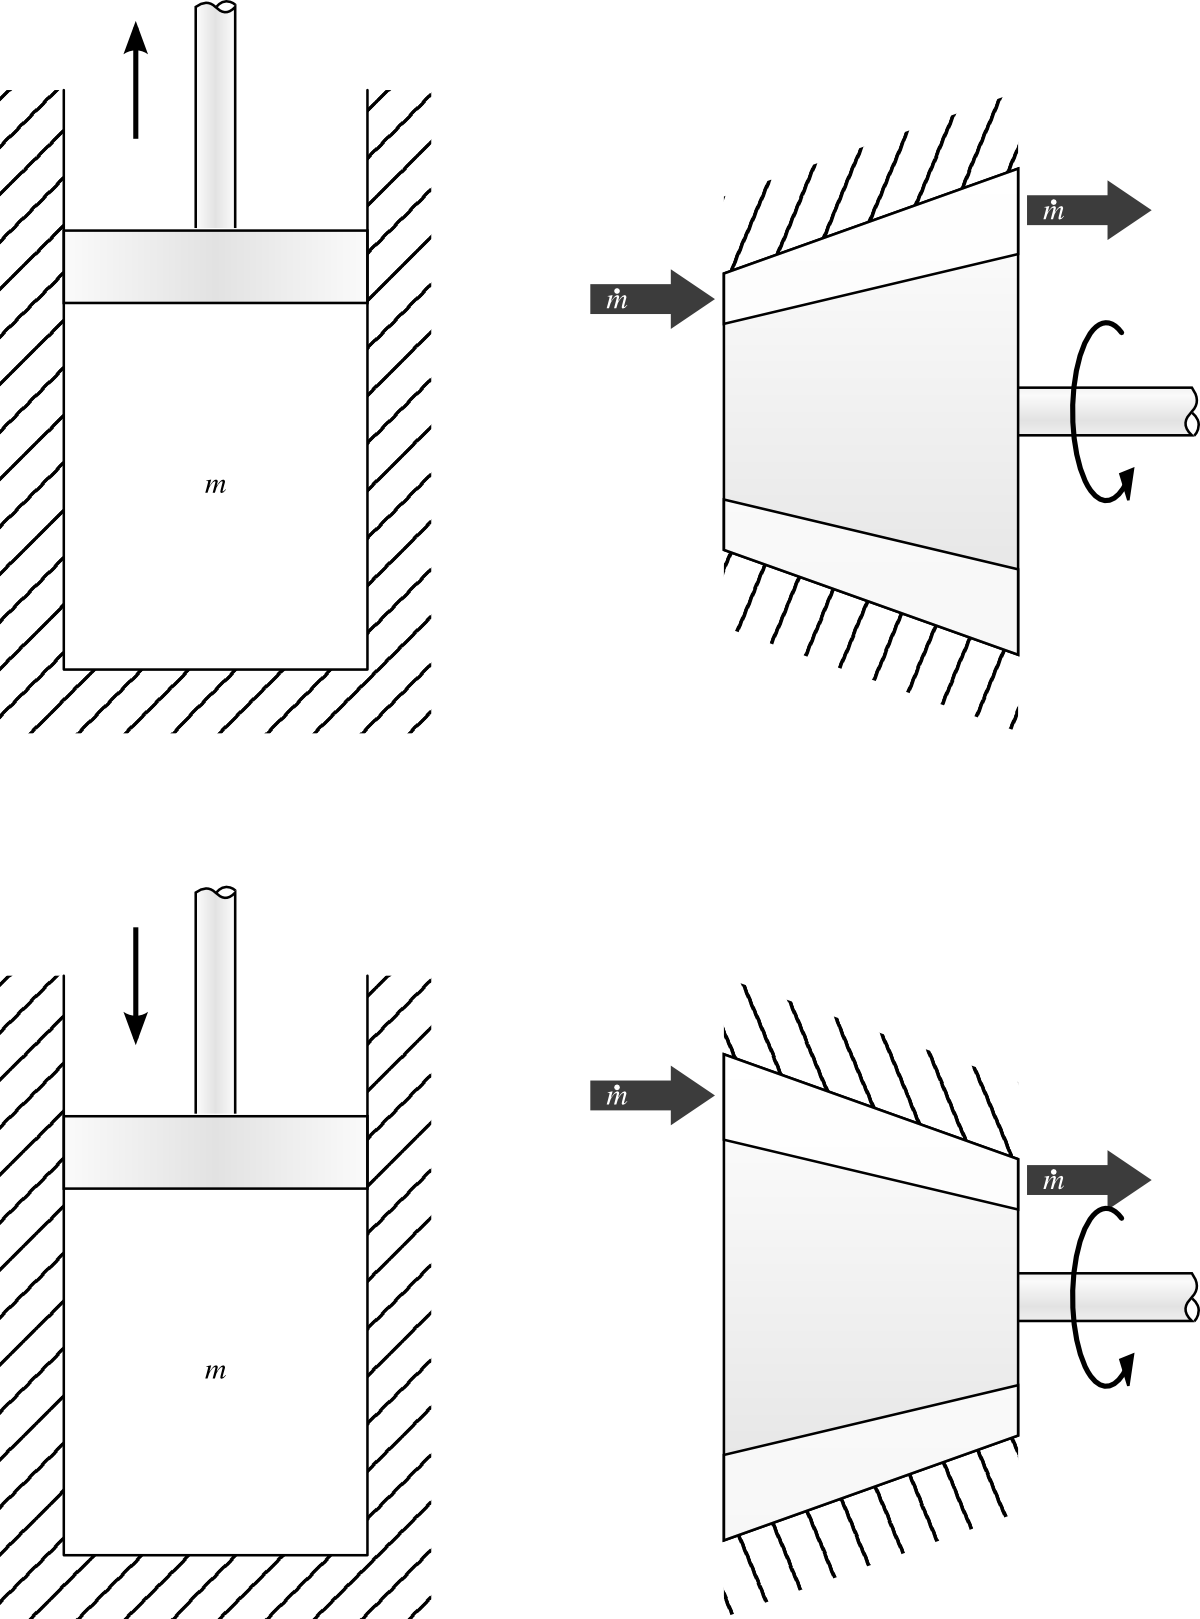
\includegraphics[width=10cm]{images/isentropique.png}
			\end{center}
			\caption{Évolution adiabatique réversible (isentropique) d’un gaz parfait. En système fermé (à gauche) comme en système ouvert (à droite), l’appareil est parfaitement isolé, de sorte qu’il n’y ait aucun transfert de chaleur, même si la température du gaz varie.}
			\label{fig_gp_isentropique}
		\end{figure}
		
	
		Une évolution \vocab{adiabatique réversible} est effectuée infiniment lentement. Un piston dans un cylindre devra pour cela être déplacé infiniment lentement, et un compresseur en flux continu devra pour cela être infiniment long. Plus tard, dans le \courshuit, nous appellerons ces transformations \vocab{isentropiques}.

		\begin{figure}
			\begin{center}
				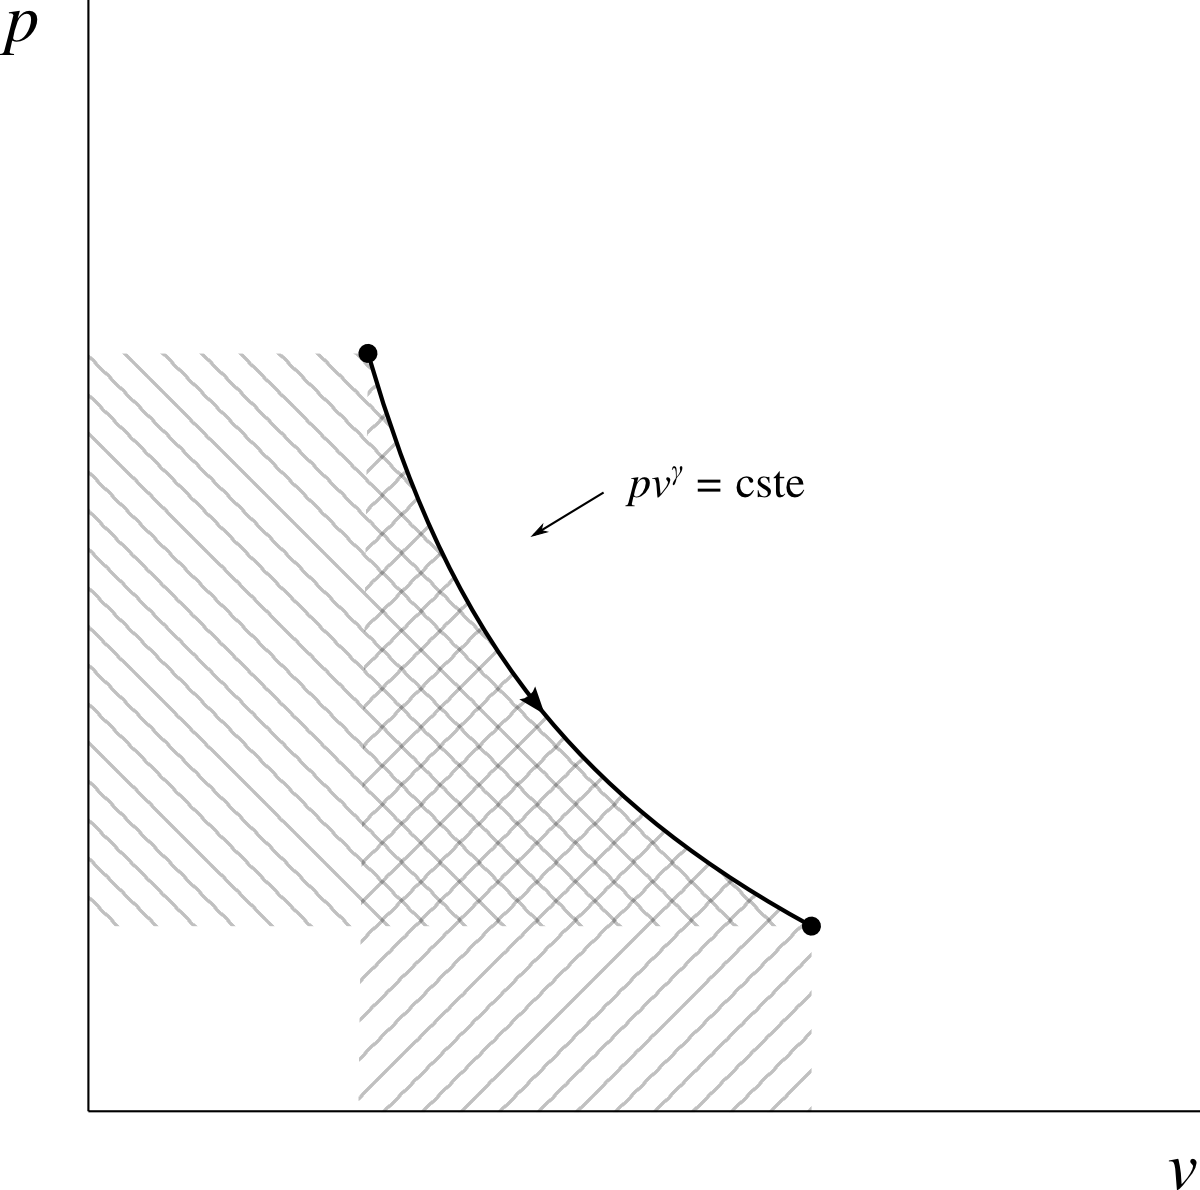
\includegraphics[width=8cm]{images/pv_isentropique.png}
			\end{center}
			\caption{Détente adiabatique réversible d’un gaz parfait, représentée sur un diagramme pression-volume.}
			\label{fig_gp_isentropique_pv}
		\end{figure}

		
		En système fermé, nous avons $q_{1\to2} + w_{1\to2} = \Delta u$, et, si l’évolution est réversible, la chaleur et le travail sont quantifiés sans la moindre difficulté :
		
		\begin{equation}
			q_{1\to2} = 0
		\end{equation}
		\begin{equationterms}
			\item lors d’une évolution adiabatique réversible, par définition.
		\end{equationterms}
		
		
		\begin{IEEEeqnarray}{rCl}
			w_{1\to2} 	& = & \Delta u - q_{1\to2} = \Delta u  \nonumber \\
			w_{1 \to 2} 	& = & c_v \ \Delta T
			\label{eq_gp_travail_isentropique_sf}
		\end{IEEEeqnarray}
		\begin{equationterms}
			\item lors d’une évolution adiabatique réversible en système fermé.
		\end{equationterms}

		
		Lorsque l’évolution se fait en système ouvert, nous avons $q_{1\to2} + w_{1\to2} = \Delta h$, et nous pouvons de même écrire :
		
		\begin{IEEEeqnarray}{rCl}
			q_{1\to2} 	& = & 0 	\\
			w_{1\to2} 	& = & c_p \ \Delta T
			\label{eq_gp_travail_isentropique_so}
		\end{IEEEeqnarray}
		\begin{equationterms}
			\item lors d’une évolution adiabatique réversible, en système ouvert.
		\end{equationterms}

		
		
		Malheureusement, ces deux équations~\ref{eq_gp_travail_isentropique_sf} et~\ref{eq_gp_travail_isentropique_so} ne sont d’aucune utilité tant que l’on a pas prédit la température $T_2$ à la fin de l’évolution. Or, dans une évolution adiabatique réversible, rien ne reste constant : le volume spécifique, la pression et la température varient tous les trois. Comment quantifier ces propriétés ?
		
		
		Partons d’une évolution adiabatique infiniment courte dans un système fermé. Lorsque l’évolution est réversible, $\diff w = -p \diff v $ et alors :

		\begin{IEEEeqnarray*}{rCl}
			\diff q = \diff u - \diff w 	& = & 0		\nonumber \\
			\diff u + p \diff v  		& = & 0
		\end{IEEEeqnarray*}

		Comme $\diff u = c_v \diff T$ pour un gaz parfait et que $p = R T/v $, on peut ré-écrire cette équation ainsi :

		\begin{IEEEeqnarray*}{rCl}
			c_v \diff T + \frac{R T}{v} \diff v  				& = & 0	\nonumber \\
			\frac{1}{T} \diff T + \frac{R}{c_v} \frac{1}{v} \diff v  	& = & 0
		\end{IEEEeqnarray*}
	
		En intégrant entre deux états 1 et 2 :

		\begin{IEEEeqnarray}{rCl}
			\ln \left( \frac{T_2}{T_1} \right) + \frac{R}{c_v} \ln \left( \frac{v_2}{v_1} \right) 	& = & 0	\nonumber \\
			\ln \left( \frac{T_2}{T_1} \right) + \ln \left( \frac{v_2}{v_1} \right)^{\frac{R}{c_v}} 	& = & 0	\nonumber \\
			\ln \left( \frac{T_2}{T_1} \right) & = & \ln \left( \frac{v_1}{v_2} \right)^{\frac{R}{c_v}}
			\label{eq_tmp_isentropique}
		\end{IEEEeqnarray}
	
		Et comme $R = c_p-c_v$ (\ref{eq_sectionmathschiante_2}) et $\gamma \equiv c_p/c_v$ (\ref{def_gamma}), on a $\frac{R}{c_v} = \gamma -1$, ce qui permet de reformuler l’\cref{eq_tmp_isentropique} ci-dessus :
		\begin{equation*}
			\left( \frac{T_2}{T_1} \right) = \left(\frac{v_1}{v_2} \right)^{\gamma -1}
		\end{equation*}
	
		Nous avons donc lié température et volume spécifique lorsque l’évolution est adiabatique réversible (privée d’échange de chaleur, et infiniment lente).

		Quelques manipulations algébriques, qu’il est laissé à l’étudiant/e de réviser, nous permettent de décliner cette expression en fonction de la pression, et on obtient donc les trois relations :

		\begin{IEEEeqnarray}{rCl}
			\left( \frac{T_1}{T_2} \right)	& = & \left( \frac{v_2}{v_1} \right)^{\gamma -1}		\label{eq_isentropique_horrible1}\\
			\left( \frac{T_1}{T_2} \right)	& = & \left( \frac{p_1}{p_2} \right)^{\frac{\gamma -1}{\gamma}}	\label{eq_isentropique_horrible2}\\
			\left( \frac{p_1}{p_2} \right)	& = & \left( \frac{v_2}{v_1} \right)^{\gamma}			\label{eq_isentropique_horrible3}
		\end{IEEEeqnarray}

		\begin{equationterms}
			\item pour toute évolution adiabatique réversible.
		\end{equationterms}

		Cette dernière \cref{eq_isentropique_horrible3} équivaut à l’expression :
		\begin{equation}
			p v^{\gamma} = \text{constante}
			\label{eq_isentropique_horrible3bis}
		\end{equation}

		\begin{equationterms}
			\item pour toute évolution adiabatique réversible.
		\end{equationterms}

		Nous disposons donc d’une relation simple entre pression et volume pour un gaz parfait suivant une évolution réversible adiabatique ; chaque gaz possédant sa propre valeur de $\gamma$. Remarquons une dernière fois que même si par définition aucune chaleur n’est échangée, la température varie systématiquement, comme l’indique la relation~\ref{eq_isentropique_horrible1}.

		
	\subsection{Évolutions arbitraires}
	
		Il faut bien garder en tête que l’on peut en pratique faire évoluer les propriétés d’un gaz \emph{de n’importe quelle façon arbitraire} (\cref{fig_gp_pv_coeur}).
		
		\begin{figure}
			\begin{center}
				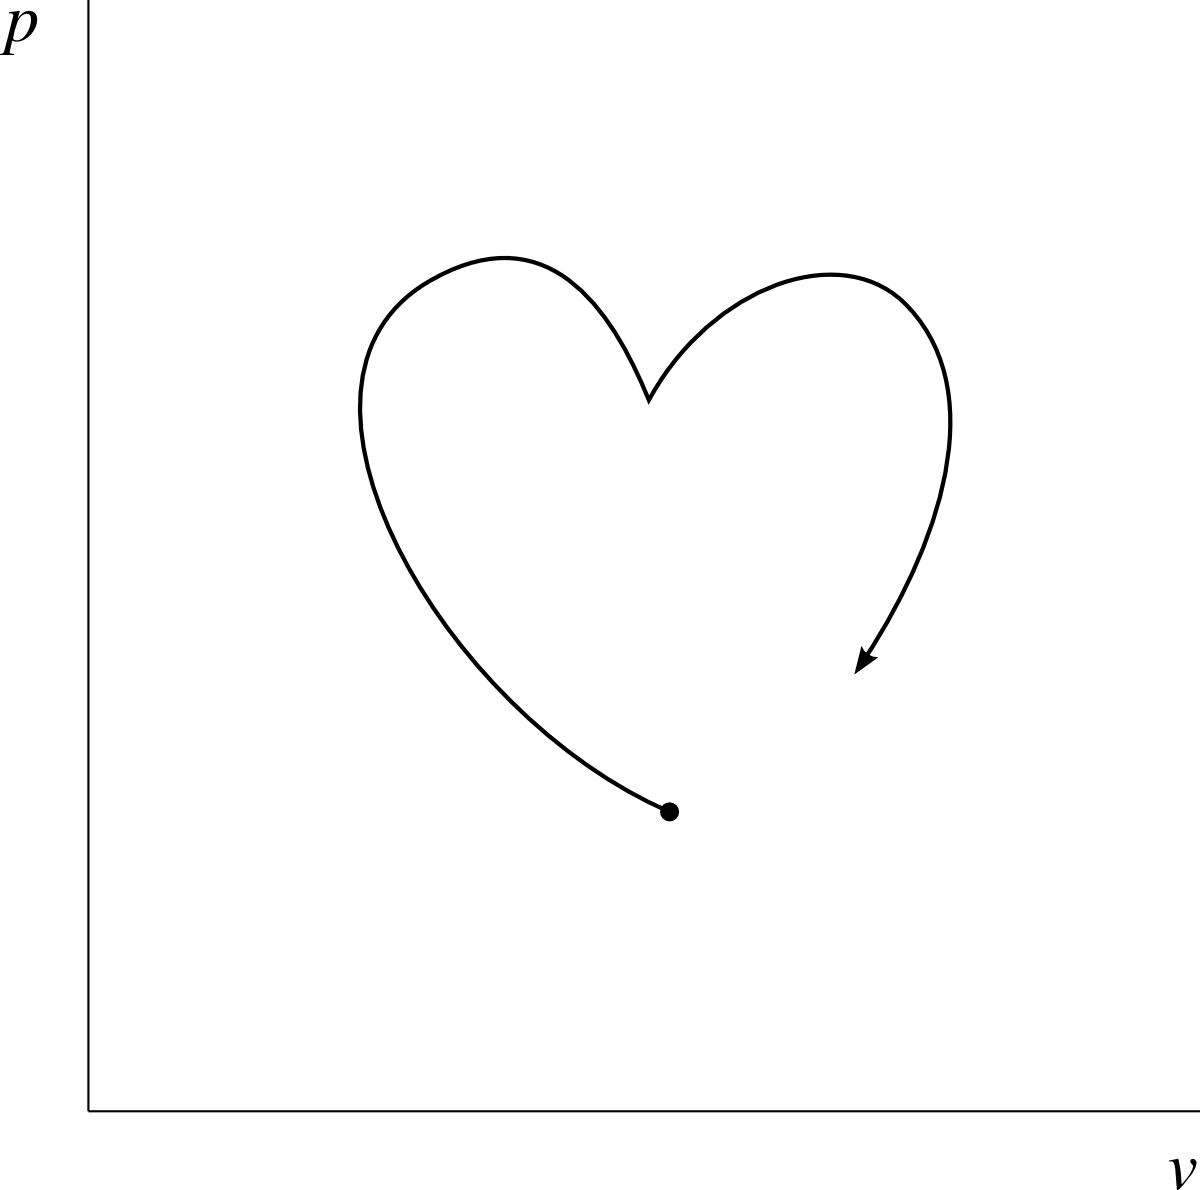
\includegraphics[width=8cm]{images/pv_coeur.png}
			\end{center}
			\caption{Évolution entièrement arbitraire d’un gaz parfait représentée sur un diagramme pression-volume. Une telle évolution requiert une combinaison complexe de transferts de chaleur et de travail, que l’étudiant/e est invité/e à se représenter.}
			\label{fig_gp_pv_coeur}
		\end{figure}
		
		Nous nous sommes concentrés sur quatre évolutions particulières des gaz parfaits, parce qu’elles jouent chacune un rôle important, pour les physiciens et pour les ingénieurs, dans la conception des machines thermiques. En contrôlant astucieusement les transferts de chaleur et de travail, on peut bien sûr provoquer n’importe quelle évolution arbitraire.
